\documentclass[%
	%draft,
	paper=a4,%
	abstract=true,%
	]{scrartcl}

\usepackage[utf8]{inputenc}
\usepackage[english]{babel}
\usepackage{graphicx}	
\usepackage{ifpdf}
\ifpdf
	\usepackage{setspace}
		%\doublespacing
	\usepackage{microtype}
	\usepackage[colorinlistoftodos]{todonotes}
\else
	\DeclareGraphicsExtensions{.png}
	\usepackage[disable]{todonotes}	
\fi	
\usepackage[load-configurations=binary]{siunitx}
	\DeclareSIUnit\Molar{\textsc{m}}
\usepackage{svn-multi}
\usepackage{subfig}
\usepackage{booktabs}
\usepackage{fancyhdr}
\usepackage{tikz}
\usepackage{pgfplots}
\usepackage[numbers,square,sort&compress]{natbib}
\usepackage{scrtime}
\usepackage[version=3]{mhchem}
\usepackage{lastpage}	
\usepackage{xspace}
\usepackage[autostyle=true]{csquotes}
%\usepackage{endfloat}
\usepackage{hyperref}

% Subversion Information
\svnidlong
{$HeadURL$}
{$LastChangedDate$}
{$LastChangedRevision$}
{$LastChangedBy$}
\svnid{$Id$} 
 
\pagestyle{fancy}
\fancyfoot{}
\fancyfoot[OR]{\tiny Typeset on \today\ at \thistime\ from \href{\svnkw{HeadURL}}{SVN-Version \svnkw{LastChangedRevision}} | Page \thepage\ of \pageref{LastPage}}
\fancyfoot[EL]{\tiny Page \thepage\ of \pageref{LastPage} | Typeset on \today\ at \thistime\ from \href{\svnkw{HeadURL}}{SVN-Version \svnkw{LastChangedRevision}}}
 
\newcommand{\imsize}{\linewidth}
\newlength\imagewidth		% needed for scalebars
\newlength\imagescale		% ditto

\newcommand{\footremember}[2]{\footnote{#2}\newcounter{#1}\setcounter{#1}{\value{footnote}}}
\newcommand{\footrecall}[1]{\footnotemark[\value{#1}]}

\newcommand{\superscript}[1]{\ensuremath{^{\textrm{#1}}}}
\newcommand{\subscript}[1]{\ensuremath{_{\textrm{#1}}}}

\newcommand{\ie}{i.\,e.\xspace}
\newcommand{\eg}{e.\,g.\xspace}
\newcommand{\twod}{2\textsc{d}\xspace}
\newcommand{\threed}{3\textsc{d}\xspace}

\newcommand{\subfigureautorefname}{\figureautorefname} % make \autoref work with \subfloat
 
\title{How to stereologically characterize individual acini in tomographic datasets of rat lungs\todo{Title: max.\ 160 characters, currently 89.}}
\subtitle{Stereological characterization of individual rat lung acini\todo{Running Head: max.\ 60 char., currently 59.}}

\author{%
	David Haberthür\footremember{ana}{Institute of Anatomy, University of Bern, Switzerland}%
	\and Sébastien Barré\footrecall{ana}%
	\and Stefan Tschanz(?)\footrecall{ana}%
	\and Lilian Salm(?)\footrecall{ana}%
	\and Marco Stampanoni\footremember{psi}{Swiss Light Source, Paul Scherrer Institut, Villigen, Switzerland}\ \footremember{eth}{Institute for Biomedical Engineering, Swiss Federal Institute of Technology and University of Zürich, Switzerland}%
	\and Johannes C. Schittny\footrecall{ana}\ \footremember{contact}{Corresponding Author: Email: \href{mailto:schittny@ana.unibe.ch}{schittny@ana.unibe.ch}, Telephone: +41 31 631 46 35, Fax: +41 31 631 38 07, Address: Institute of Anatomy, University of Bern, Baltzerstrasse 2, CH-3012 Bern}%
	}

\begin{document}
\setcounter{secnumdepth}{-1} % No section numbering, please!
\renewcommand{\subsectionautorefname}{\sectionautorefname} % useful for \autoref
\renewcommand{\subsubsectionautorefname}{\sectionautorefname} % useful for \autoref
\maketitle
\begin{center}
\vfill
Typeset on \today\ at \thistime\ from Rev \svnkw{LastChangedRevision} (\svnday.\svnmonth.\svnyear\ \svnhour:\svnminute)
\vfill
To appear in \emph{\href{http://jap.physiology.org/}{Journal of Applied Physiology}}, \emph{Innovative Techniques}
\vfill
\end{center}
\clearpage

\begin{abstract}
The pulmonary acinus represents the functional unit of the lung. Due to a restricted availability of high resolution imaging methods the knowledge about the development of the pulmonary acini is limited. Using synchrotron radiation based tomographic microscopy we developed a method to estimate the volume of single acini throughout postnatal lung development. We developed a method to isolate and analyze single functional units of the lung, the so-called acini in three dimensions with minimal effort. In tomographic datasets acquired at the TOMCAT beamline we closed the transition between conducting and gas-exchanging airways bronchioles semi-automatically with three-dimensional discs acting as segmentation breakpoints. Our method makes it possible to extract acini for volume analysis, something which is not feasible on classic microscopy slides, since serial sectioning destroys the three-dimensional information of the dataset. The automatic volume analysis of single acini was manually confirmed with stereological assessment. Our proposed method of analyzing single functional units of the mammalian lung opens the possibility to study postnatal development of functional lung units on a large scale also because it is by magnitudes faster than manual stereological counting.\todo{One paragraph, no more than 250 words, currently 186.}
\end{abstract}

\newenvironment{keywords}{\begin{trivlist}\item[]{\bfseries\sffamily Keywords:}\ }{\end{trivlist}}
\begin{keywords}
lung development, tomography, acinus, visualization\todo{Three to five words that do not appear in the title or running head}
\end{keywords}

\clearpage
\todo{Table of contents will be removed, just for overview purposes!}
\tableofcontents

\clearpage
\section{Introduction}\label{sec:Introduction}
Due a restricted availability of high resolution three-dimensional (\threed) imaging methods the knowledge about the development of the functional unit of the lung is limited. These functional units of the lung parenchyma are the so called pulmonary acini, which correspond to the gas-exchange volume in the lung which is ventilated by one purely conducting airway~\cite{Rodriguez1987}.

Using synchrotron radiation based tomographic microscopy with enhanced field of view \cite{Haberthuer2010a} we developed a method to evaluate the volume of single acini throughout postnatal lung development. In this manuscript we present the methodology to extract single acini in high-resolution three-dimensional datasets obtained with synchrotron-radiation based tomographic microscopy.

Up to now it has not been possible to extract a large amount of single acini from physical sections of lung tissue. \citet{Woodward2005} achieved three-dimensional reconstructions of three adult ducks using manual effort to trace serial sections of the tissue. Since classic histological preparations (like cutting in a Microtome, serial sectioning, etc.) cause deformations in the sectioned tissue like compression artifacts from cutting and folding or shearing of the tissue during mounting. This essentially destroys the three-dimensional information inherent in successive slices of the lung structure. Such a destruction makes it impossible to observe and trace single acini to extract their volume. Tomographic imaging of the lung tissue preserves this three-dimensional structure, since the slices through the tissue are entirely virtual and thus makes it possible to observe the volume of single acini.

Through careful segmentation we can then extract single functional lung units---the so-called acini---and analyze those with classic and accepted methods in both two and three dimensions. In addition to three-dimensional volume analysis in a visualization software we used standard stereological analysis \cite{Hsia2010} as a gold-standard to compare our results with a ground truth. As stated by \citet{Hsia2010}, Stereology refers to the mathematical methods for analyzing these properties of an irregular three-dimensional structure using two-dimensional planar sections obtained by physical or optical imaging techniques.

Extracting single functional lung units from the tomographic datasets enabled us to perform such a stereological analysis to obtain a complete description of the functional lung units including alveolar number, surface and volume and compare these values over the course of the postnatal lung development. Such a complete description is only possible with tomographic data, since the three-dimensional information in the sample is not destroyed.

As \citet{Schittny2007a} described, descriptions of the stages of lung development are based on light microscopical observations of morphological changes in the developing lung. In this manuscript, we present a method to analyze and describe the postnatal development of the functional units of the lung, \ie changes in their volume and surface.

\subsection{Lung structure and the functional units of the lung}
The airway structure of the mammalian lung is formed from dichotomous branches~\cite{Weibel1991}, starting from the trachea. The first branching generations lead into the bronchi. With increasing depth into the airway tree, the airway diameter of the airways is reduced, the bronchi are divided into bronchioles, leading to the terminal bronchioles which mark the end of the pipe-like purely conducting airways. The respiratory bronchioles mark the start of the gas-exchange region in the lung. We start to see changes in the airway wall structure---alveolar outpouchings---which mark the change between purely conducting and gas-exchanging airways (see \autoref{fig:ManholeCoverExplanation}). After this point, the so-called acinar airways and the acinus---the functional unit of the lung---begin. The observation of such changes in the airway wall make it possible to extract single acini from the three-dimensional tomographic datasets, as described later in Materials and Methods.

The lung structure can be assessed using stereology~\cite{Hsia2010}, as shown by \citet{Tschanz2002}. Such an analysis is generally based on serial sections of the sample, thus the extracted information is a two-dimensional description \blockquote[\cite{Tschanz2002}]{of the parenchymal air space geometry and, due to geometric laws, it is not allowed to extrapolate these \twod statements directly to \threed structures}. With stereological methods it is possible to extract global volume information, but it not easily possible to extract such information from a functional subunit of an organ like the acini in the lung, since it cannot easily be judged which detail on one microscopy slide belongs to which functional unit in the three-dimensional compound.

\section{Materials and Methods\label{sec:MM}}
\subsection{Rat lung samples}
Results shown in this manuscript have been obtained from lungs from adult Sprague-Dawley rats at day 60 after birth. Animals were deeply anesthetized with a mixture of Prequillan, Xylopan and Narkosan at approximately \SI{10}{\micro\litre} per \SI{35}{\gram} body weight\todo{“Type and dosage of anesthetic agent should be specified”}. Their lungs were instilled with \SI{2.5}{\percent} glutaraldehyde (\cf{CH2(CH2CHO)2}) in \SI{0.03}{\Molar} potassium-phosphate buffer (pH 7.4) at a constant pressure of \SI{20}{\centi\meter} water column. At this applied pressure, the rat lung reaches its mid-respiratory volume. The instillation was performed via tracheotomy after opening the chest cavity and setting a pneumothorax through perforation of the diaphragm. After instillation the lung was removed from the chest cavity and the instillation pressure was maintained during fixation (in the same fixative at \SI{4}{\celsius} for at least \SI{24}{\hour}) in order to prevent a recoiling of the lung. Details of the whole procedure have been described by \citet{Tschanz2002} as well as \citet{Burri1974}.

After fixation, the samples were prepared for tomographic imaging by postfixation with \SI{1}{\percent} osmium tetroxide (\cf{OsO4}) and staining with \SI{4}{\percent} uranyl nitrate (\cf{UO2(NO3)2}) to increase the x-ray absorption contrast. Using Histoclear (Merck KGaA, Darmstadt, Germany) as an intermedium the samples were then dehydrated in a graded series of ethanol and embedded in paraffin prior to mounting them onto standard scanning electron microscopy sample holders (PLANO GmbH, Wetzlar, Germany) with paraffin~\cite{Tsuda2008}.

The handling of animals before and during the experiments, as well as the experiments themselves, were approved and supervised by the Swiss Agency for the Environment, Forests and Landscape and the Veterinary Service of the Canton of Bern, Switzerland.

\subsection{Tomographic data acquisition\label{sec:tomcat}}
The tomographic experiments were performed at the \href{http://www.psi.ch/sls/tomcat/}{TOMCAT beamline} at the \href{http://www.psi.ch/sls/}{Swiss Light Source}, \href{http://www.psi.ch/}{Paul Scherrer Institut}, Villigen, Switzerland~\cite{Stampanoni2006a}. The samples were scanned at \SI{20.0}{\kilo\electronvolt} corresponding to a wavelength of \(\lambda=\SI{0.62}{\angstrom}\). % \lambda = 1.24e-6 eV/m / 20 keV = 6.197796e-11 m = 0.6197796 Ångström
After penetration through the sample, the x-rays were converted into visible light by a \SI{20}{\micro\meter} thick LuAG:Ce scintillator (Lutetium Aluminum Garnet activated by cerium, \cf{Lu3Al5O12}, \href{http://www.crytur.cz/}{Crytur Ltd.}, Turnov, Czech Republic).

A 10\(\times\) magnifying, diffraction limited microscope optics was used to magnify the image onto a \SI{18}{\micro\meter} thick Cerium doped Yttrium Aluminium Garnet (YAG) (\cf{Y3Al5O12}) scintillator screen. Subsequently, a high-resolution 2048\(\times\)2048 pixel CCD camera (\href{http://www.pco.de/sensitive-cameras/pco2000/}{pco.2000}, \href{http://www.pco.de/}{PCO AG}, Kelheim, Germany) with \SI{14}{\bit} dynamic range was used to digitize this magnified image. To reduce imaging noise and increase the acquisition speed, we operated the detector in 2\(\times\)2 binning mode. As a result, the pixel size was \SI{1.48}{\micro\meter} and the exposure time was between \SIrange{160}{180}{\milli\second}. Details of the TOMCAT beamline setup have been thoroughly described by \citet{Stampanoni2006a}.

To be able to safely distinguish the alveolar septa which in rats have an mean thickness of \SIrange{5}{10}{\micro\meter} (calculated from data in \citet{Burri1974}) the tomographic images used for analysis of the functional units of the lung need to have a resolution in the order of one to two microns. Since we selectively wanted to extract a large amount of single acini, we not only needed to acquire high resolution tomographic scans, but also acquire dataset with both large volume and in high resolution. Usually---with classic microscopy based imaging methods---a large field of view can only be acquired with low magnification and vice-versa. Since the our samples were larger than the classic field of view of TOMCAT at the aforementioned optical properties (\(1.52\times1.52\times\SI{1.52}{\milli\meter}\)) we would not have been able to image the full volume of our samples. To overcome this problem, we enhanced the enhance the field of view of the TOMCAT beamline at the chosen optical configuration. This enhancement was done with the so called wide field scanning protocol, described by \citet{Haberthuer2010}.

Briefly summarized, the wide field scanning process merges three or five independently acquired partial tomographic scans which successively cover the total desired field of view. The single projections of the are merged to one large projection spanning the desired field of view on during tomographic reconstruction. This merging is performed on the tomographic reconstruction cluster of seven \SI{64}{\bit} Opteron machines with four cores and \SI{8}{\giga\byte} RAM each. Implementing the merging on the cluster made it possible to use the classic tomographic reconstruction work flow at TOMCAT, which has been described in detail by \citet{Hintermueller2010}.

Using this wide field scanning approach we increased the lateral field of view at TOMCAT three-fold, while keeping both voxel size and reconstruction quality on the desired level and avoiding the aforementioned trade-off between voxel size and sample volume. Since we also performed a so called stacked scan in relation to the z-axis of the tomographic setup, we even further increased the field of view and the recorded volumes of our samples. We acquired tomographic dataset of approximately 3000\(\times\)3000\(\times\)3072 pixels with \SI{1.48}{\micro\meter} pixel size. This corresponds to a 9-fold increase in recorded volume as compared to a classic scan at TOMCAT, giving us the advantage of both high resolution images and large visible sample volume to extract the single functional lung units.

\subsection{Visualization and Extraction of Acini}
The tomographic datasets of the sample were three-dimensionally analyzed and visualized using \href{http://mevislab.de}{MeVisLab} (Version 2.1 (2010-07-26 Release)~\cite{Bitter2007}, MeVis Medical Solutions AG and Fraunhofer MEVIS - Institute for Medical Image Computing, Bremen, Germany). The analysis and visualizations have been performed on a Dell Precision T7500 work station (\SI{24}{\giga\byte} RAM, Intel Xeon CPU X5550 at \SI{2.66}{\giga\hertz}, Windows 7 Professional \SI{64}{\bit}). 

The tomographic datasets obtained at TOMCAT were converted from a stack of TIFF-files to the native GVR format of MeVisLab, a multi-resolution \href{https://secure.wikimedia.org/wikipedia/en/w/index.php?title=Octree&oldid=409131920}{octree}-based image format. This permitted us to easily switch between resolutions in the dataset to interactively perform the visualization and preliminary analysis on a lower resolution prior to the final analysis on full resolution datasets. A graphical user interface was developed using MDL (MeVisLab Definition Language) to facilitate the task of defining regions of interest in the dataset, isolating single functional lung units, extracting them from the tomographic dataset for subsequent verification, visualizing the extracted acini in \threed, analyzing and tabulating their volume.

\subsubsection{Manhole Covers\label{sec:manholecovers}}
On binned datasets we extracted conducting airway segments using a threshold interval based region growing algorithm~\cite{Zucker1976}. A seed point for the region growing algorithm was manually defined inside the terminal bronchiole or alveolar duct on one of the most proximal slices of the dataset (shown in \autoref{subfig:sample}). This approach made it possible to extract a connected airway segment, which was then further subdivided into conducting and gas-exchanging airways. This division was performed with manually placed circular segmentations stoppers, which we dubbed manhole covers (shown as red discs in \autoref{subfig:airway segment} and \subref*{subfig:extracted acini}). The manhole covers were implemented through a \href{http://www.mevis-research.de/cgi-bin/discus/board-auth.cgi?lm=1282233250&file=/839/11760.html}{custom module (\emph{XMarkerClipPlanes})} written by Milo Hindennach, a member of the MeVis Developer team. These segmentations stoppers manhole covers were manually placed in the airway segment based on morphological criteria, \ie on changes in the airway wall structure which mark the entrance point into the acinus.

\renewcommand{\imsize}{\linewidth}
\begin{figure}
	\centering
	\pgfmathsetlength{\imagewidth}{\imsize}%
	\pgfmathsetlength{\imagescale}{\imagewidth/1207}%
	\def\x{746}% scalebar-x at golden ratio of x=1207px
	\def\y{922}% scalebar-y at 90% of height of y=1024px
	\begin{tikzpicture}[x=\imagescale,y=-\imagescale]
		\node[anchor=north west, inner sep=0pt, outer sep=0pt] at (0,0) {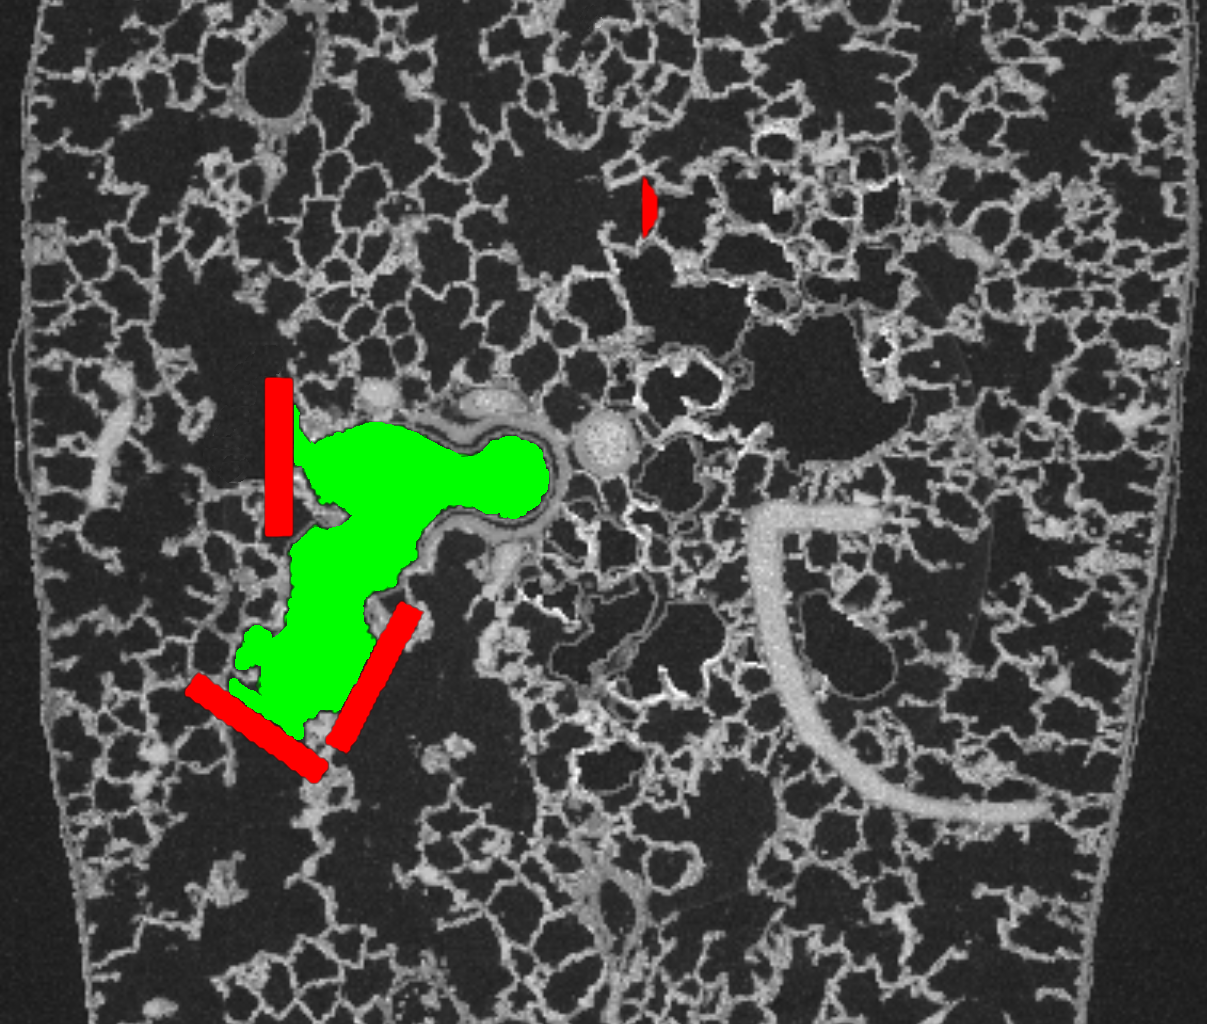
\includegraphics[width=\imagewidth]{img/ManholeCoverExplanation/60d_2_no_markers_crop}};
		% 267px = 0.5mm > 100px = 187um > 267px = 500um, 53px = 100um
		\draw[|-|,white, thick] (\x,\y) -- (\x+267,\y) node [midway, above] {\SI{500}{\micro\meter}};
		\draw[yellow,dashed,ultra thick] (192,385) circle (40);
		\draw[yellow,dashed,ultra thick] (278,296) circle (40);
		\draw[yellow,dashed,ultra thick] (340,758) circle (30);
		%\draw[yellow,dashed,ultra thick] (334,822) circle (30);
		\draw[yellow,dashed,ultra thick] (326,870) circle (30);
		\draw[yellow,dashed,ultra thick] (300,806) circle (30);
	\end{tikzpicture}%
	\caption{One slice of a tomographic dataset showing an extracted conducting airway (green) and manhole cover (red). The dashed yellow circles highlight examples of outpouchings of the airway wall which mark the change from conducting to gas-exchanging regions. Additionally, changes in the epithelial layer of the airway wall, especially changes in thickness and structure also mark this change. Visually assessing these changes made it possible to semiautomatically place manhole covers in the \threed tomographic dataset to isolate single acini from our dataset. Three manhole covers (red) are shown cut right through the middle, a fourth (upper middle) is only partially shown on this slice.}
	\label{fig:ManholeCoverExplanation}
\end{figure}

Using a separate region growing module, we subsequently and automatically extracted single acini from the datasets (shown as yellow volumes in \autoref{subfig:extracted acini}). Since the manhole covers placed in the first step are defined through their diameter and \href{https://secure.wikimedia.org/wikipedia/en/w/index.php?title=Surface_normal&oldid=411684319}{surface normal} we were able to automatically define the seed point for the additional region growing modules used for the extraction of the single acini. We simply flipped the direction of the surface normal and placed the seed point along this vector slightly behind the manhole cover, inside the acinar airspace. The only manual work left was the iterative selection of the correct gray value threshold used for the region growing segmentation and the tabulation of the automatically calculated acinar volume.

\renewcommand{\imsize}{.333\linewidth}%
\pgfmathsetlength{\imagewidth}{\imsize}%
\pgfmathsetlength{\imagescale}{\imagewidth/1008}%
\def\x{50}% scalebar-x at golden ratio of x=1008px
\def\y{916+20}% scalebar-y at 90% of height of y=1018px
\begin{figure}
	\centering
	\subfloat[Sample]{%
		\begin{tikzpicture}[x=\imagescale,y=-\imagescale]
			\node[anchor=north west, inner sep=0pt, outer sep=0pt] at (0,0) {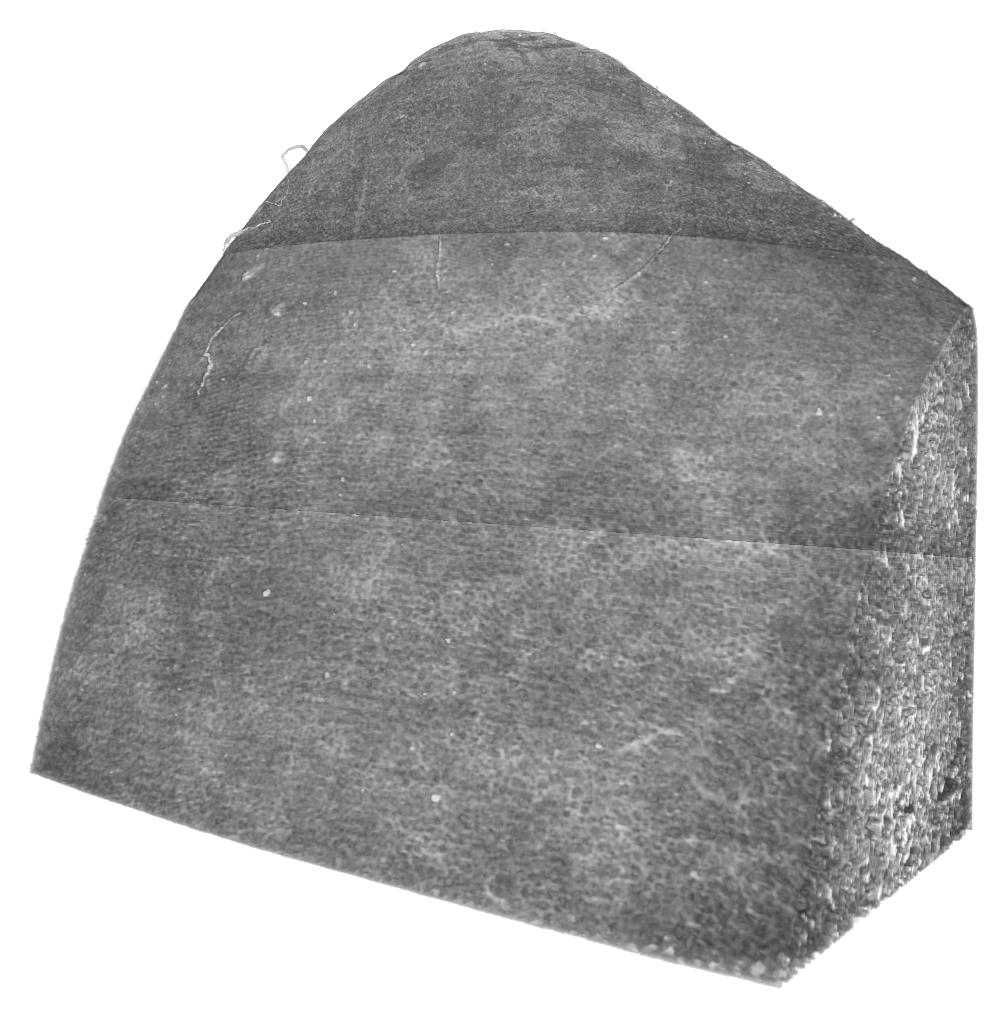
\includegraphics[width=\imagewidth]{img/ManholeCover/R108C60B_2010c_Acinus_Sample}};
			% 774px = 4.363mm > 100px = 564um > 89px = 500um, 18px = 100um
			%\draw[|-|,blue,thick] (775,990) -- (33,771) node [sloped,midway,above,fill=white,semitransparent,text opacity=1] {\SI{4.363}{\milli\meter} (2948px) TEMPORARY!};
			\draw[|-|, thick] (\x,\y) -- (\x+89,\y) node [right] {\SI{500}{\micro\meter}};
		\end{tikzpicture}%
		\label{subfig:sample}%
		}%
	\subfloat[Extracted conducting airways with manhole covers shown overlayed over Sample.]{%
		\begin{tikzpicture}[x=\imagescale,y=-\imagescale]
			\node[anchor=north west, inner sep=0pt, outer sep=0pt] at (0,0) {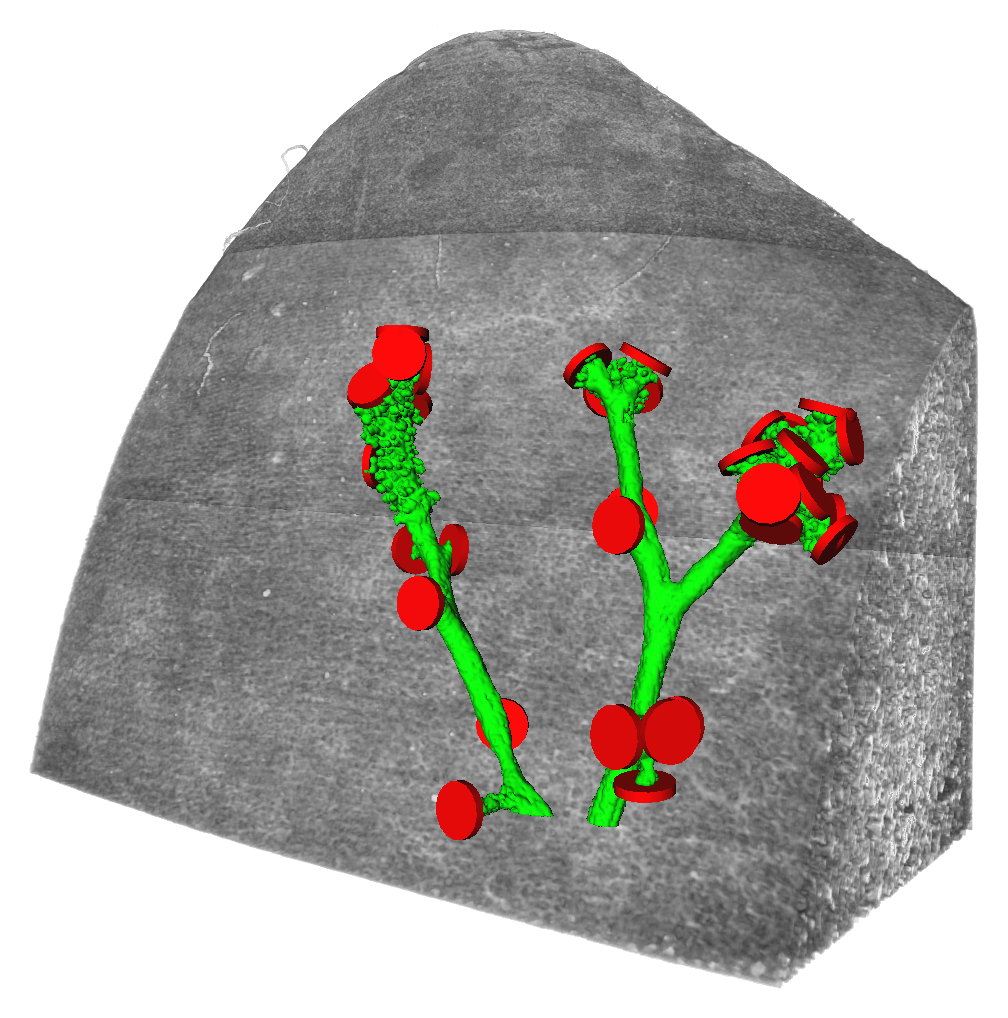
\includegraphics[width=\imagewidth]{img/ManholeCover/R108C60B_2010c_Acinus_Airspace_Overlay}};
			\draw[|-|, thick] (\x,\y) -- (\x+89,\y) node [right] {\SI{500}{\micro\meter}};
		\end{tikzpicture}%
		\label{subfig:airway segment}%
		}%
	\subfloat[Extracted acini.]{%
		\begin{tikzpicture}[x=\imagescale,y=-\imagescale]
			\node[anchor=north west, inner sep=0pt, outer sep=0pt] at (0,0) {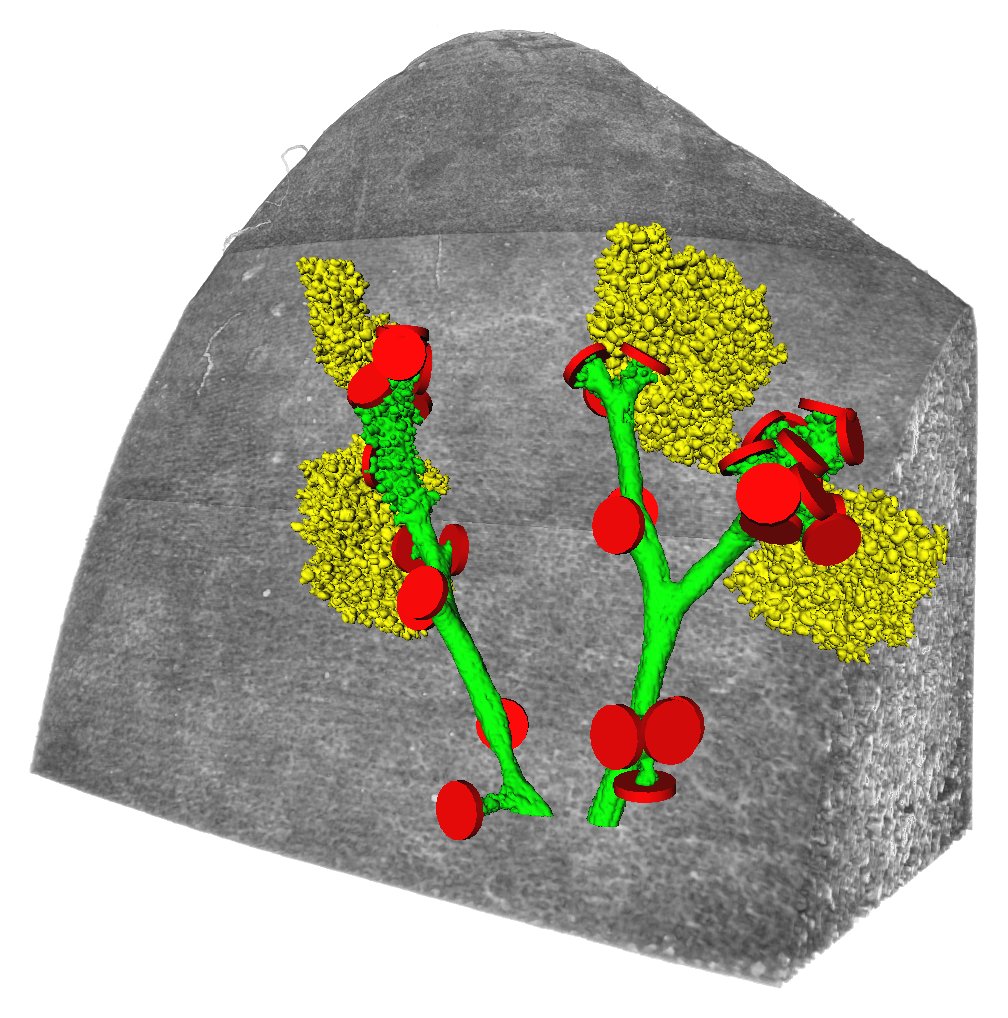
\includegraphics[width=\imagewidth]{img/ManholeCover/R108C60B_2010c_Acinus_OverlayNonTransparent}};
			% 774px = 4.363mm > 100px = 564um > 89px = 500um, 18px = 100um
			\draw[|-|, thick] (\x,\y) -- (\x+89,\y) node [right] {\SI{500}{\micro\meter}};
		\end{tikzpicture}%
		\label{subfig:extracted acini}%
		}
	\caption{Visualization of the work flow for the extraction of the acinar volumes on a rat lung sample extracted at day 60: %
		\subref{subfig:sample}: \threed visualization of a sample. To increase the field of view nine-fold compared to a classic scan at TOMCAT we stacked three wide field scans on top of each other. The borders between the three stacked scans are faintly visible as darker lines, but are only visible in this \threed visualization and did not influence the \threed reconstruction. %
		\subref{subfig:airway segment} Extracted airway segment (green) superimposed on the sample. Using a threshold based region growing algorithm, we extracted conducting airways inside the sample. The red discs shown are the so-called manhole covers, which were semiautomatically placed and used as segmentation stoppers for the region growing. %
		\subref{subfig:extracted acini} Extracted acini (yellow). Multiple extracted acini are shown superimposed over the sample in \threed. For each such acinus we recorded the volume.%
		}
	\label{fig:workflow}
\end{figure}

The volume of the single acini was calculated by multiplying the amount of segmented voxels with the voxel volume, tabulated in Excel-Files and prepared for analysis. The segmented acini were also exported as single \href{https://secure.wikimedia.org/wikipedia/en/w/index.php?title=Digital_Imaging_and_Communications_in_Medicine&oldid=415023605}{DICOM} stacks for further processing as described below.

\subsection{Stereological Analysis}
We stereologically analyzed the extracted acini according to the official research policy statements of the American Thoracic Society/European Respiratory Society, as defined by \citet{Hsia2010}. Stereological analysis refers to mathematical methods for defining physical properties of irregular \threed structures with \twod sections, obtained \eg by tomographic imaging. Stereological measurements and results are often based on simple counts of interaction between structures of interest and geometric probes, in our case points and lines. To guarantee accurate and unbiased results, we standardized each step of tissue fixation, processing sampling and analysis.

\subsubsection{Comparison of Volumes from MeVisLab with STEPanizer}
As mentioned above, the volume of the single acini was calculated from the amount of segmented voxels multiplied with their size. To check these volumes against a gold standard method, we manually and stereologically assessed the volume of single acini. For this analysis, we prepared datasets in which we combined each segmented acinus with the corresponding region of interest from the original tomographic dataset, as seen in the background of \autoref{fig:STEPanizer} and exported these regions of interest as DICOM files. With a MATLAB script we padded the volumes to a square format, extracted slices in a systematically random way and exported these images to the disk as JPG sequence for analysis with the STEPanizer. 

With a MATLAB script we prepared single slices from the aforementioned DICOM-files for each acinus in a systematic random fashion and subsequently exported to single images in JPG-format for analysis. Using a web based tool developed at our institute, the so-called STEPanizer \cite[provided free of charge at \url{http://stepanizer.com}]{Tschanz2011} we analyzed the volume and surface of the extracted acini. With the STEPanizer we counted intersections of the acinar surface with geometric line probes for the surface and performed point counting to assess the volume of the extracted acini. \autoref{fig:STEPanizer} shows one such exported slice while being measured with the STEPanizer. Counting points (green three-quarter circles) and intersections (red \href{http://www.dict.cc/englisch-deutsch/I-beam.html}{I-beam}-shaped lines) are overlayed to count both the points inside the acinar volume and intersections with the acinar surface. The measurements are exported to \href{https://secure.wikimedia.org/wikipedia/en/w/index.php?title=Comma-separated_values&oldid=441921632}{csv}-delimited tables for analysis. This process made it possible to relate the automatically calculated volumes from MeVisLab to an accepted and proven gold standard stereological method.

\renewcommand{\imsize}{\linewidth}%
\begin{figure}
	\centering
	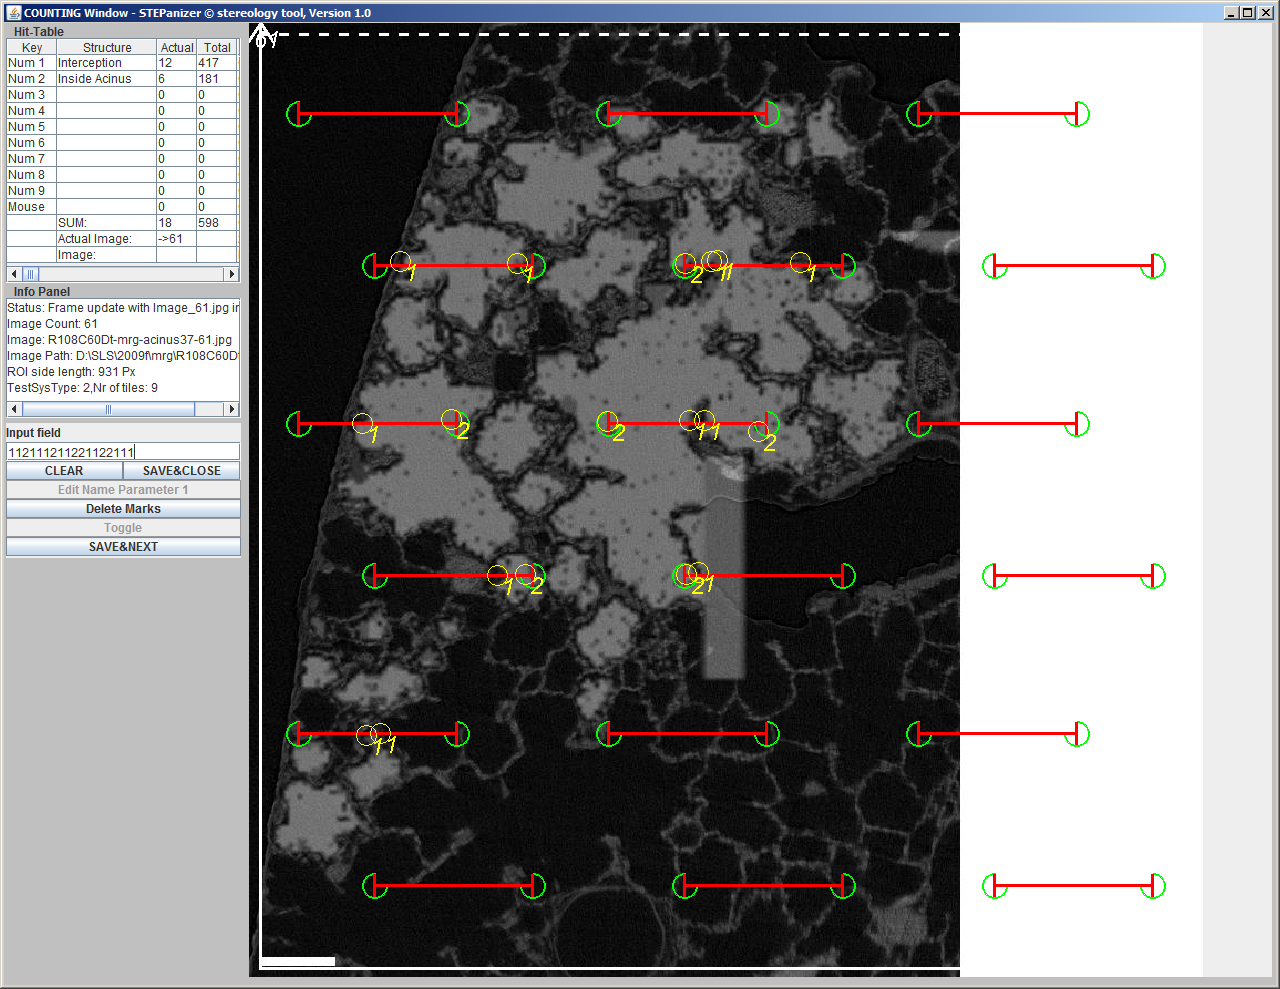
\includegraphics[width=\imsize]{img/CountingWindowSTEPanizer}
	\caption{STEPanizer counting window. The segmented acinus is visible in light gray, the manhole cover is show as rectangular darker gray (vertical slab). Both structures are overlayed and merged with the original tomographic data in the background. Line and point probes (red lines and green circles) are overlayed over the image for counting. To correctly count all structures in the image, the original non-square datasets have been padded to a square, resulting in the white rectangle at the right border of the image. Scalebar: \SI{100}{\micro\meter}.}
	\label{fig:STEPanizer}
\end{figure}

\section{Results\label{sec:Results}}
\subsection{Comparison of Volumes from MeVisLab with STEPanizer}
For four animals obtained at postnatal day 60 we isolated 165 acini. For 28 of these acini \todo{Latest numbers from ‘STEPanizerReaderAndPlotter.m’?} we compared the automatically detected volume of MeVisLab with manual stereological counting. Normalizing the volumes to the volume obtained with MeVisLab made it possible to assess differences between the two methods. The results are shown in \autoref{fig:VolumeMeVisVsSTEPanizer} \todo{Latest numbers from ‘STEPanizerReaderAndPlotter.m’?} and explained later on in the Discussion section.

\begin{figure}[htb]
	\centering
	\begin{tikzpicture}
		\begin{axis}[%
			only marks,
			legend pos=south east,
			ymin=0,
			xlabel=Acinus,
			ylabel={normalized Volume}
			]
			\addplot %[blue,mark=triangle*]
				coordinates{
					(1,100) (2,100) (3,100) (4,100) (5,100) (6,100) (7,100) (8,100) (9,100) (10,100) (11,100) (12,100) (13,100) (14,100) (15,100) (16,100) (17,100) (18,100) (19,100) (20,100) (21,100) (22,100) (23,100) (24,100) (25,100) (26,100) (27,100) (28,100)
				};
				\label{plot:mevis}				
			\addplot %[red,mark=square*]
				coordinates{
					(1,118.844) (2,118.888) (3,119.518) (4,108.54) (5,113.4) (6,115.871) (7,132.599) (8,117.926) (9,98.1566) (10,109.274) (11,129.824) (12,89.3898) (13,113.225) (14,112.215) (15,110.095) (16,102.662) (17,102.433) (18,94.6387) (19,187.167) (20,106.537) (21,159.367) (22,113.17) (23,121.325) (24,117.306) (25,94.2065) (26,135.812) (27,188.439) (28,94.0823)
				};
				\label{plot:stepanizer}
			\addplot [yellow, mark=square*] % mark=pentagon*]
				coordinates {
					(7,132.599)
					(19,187.1668)
					(21,159.3669)
					(26,135.8118)
					(27,188.439)
				};
			\label{plot:removed}
			\legend{MeVisLab, STEPanizer}				
	\end{axis} 
	\end{tikzpicture}
	\caption{Volumes of different acini estimated with different Methods. The volumes have been normalized to the volume obtained with MeVisLab (\ref{plot:mevis}). The average volume of a single acinus is \SI{10}{\percent} larger when assessed with the STEPanizer (\ref{plot:stepanizer}) as compared to MeVisLab (\SI{109.63}{\percent} vs.\ \SI{100}{\percent}). %
	See the Discussion for an explanation of the large deviations for the yellow data points (\ref{plot:removed}, values larger than \SI{130}{\percent}, removed from analysis).}
	\label{fig:VolumeMeVisVsSTEPanizer}
\end{figure}

\section{Discussion\label{sec:Discussion}}
Using a novel method dubbed manhole cover segmentation we extracted nearly 200 airway segments from 4 animals for analyzing the volume of the individual acini. With this semiautomatic method we are able to extract single functional lung units and analyze these single acini in \threed and \twod using widely accepted methods like voxel counting and Stereology. We have shown that we can automatically calculate the volume of single acini in mammalian lungs from \threed tomographic data and match the accuracy of a manual method while performing the analysis orders of magnitude faster. Only with this novel combination of methods it is possible to accurately assess the volume of single acini in \threed tomographic data.

Additionally, we used virtual \twod slices of these single acini for stereological analysis. On classic serial sections of lung tissue such an analysis is not possible since the physical cutting essentially destroys the \threed relationship between structural features in the lung parenchyma.

Our proposed method opens up the possibility to fully analyze biologically interesting parameters of the acini in the lung; extracting the volume of the acini is trivial, parameters like surface as well as number of contained alveoli and septal length per acinus can be extracted with simple stereological counting, but require manual labour. These parameters can be obtained for single acini, something which again is not possible using stereological methods on classic serial sections.

\subsection[Comparison of MeVisLab with STEPanizer]{Comparison of automatic stereology with MeVisLab and manual stereology with the STEPanizer\label{subsec:MeVisVsSTEPanizer}}
As expected, both methods show slightly different results. The automatic method based on a threshold interval region growing segmentation of the three-dimensional data in MeVisLab showed slightly lower volumes for the acini than a manual stereological analysis did. \autoref{fig:VolumeMeVisVsSTEPanizer} shows a plot of the acinar volumes normalized to the automatic method. Since the automatic calculation of the acinar volume with MeVisLab simply adds up all segmented voxels, an imprecise segmentation leads to an underestimation of the acinar volume. \autoref{fig:MeVisSegmentation} shows three exemplary slices which show large differences in volume between the two methods. Due to inevitable segmentation inaccuracies (dark spots inside the segmented acinus in \autoref{subfig:60d_acinus32} we underestimated the volumes with the automatic method compared to the manual, stereological method, where we visually discard such inaccuracies.

In some extracted acini we have seen differences in gray values in the z-direction of the stack. Since the region growing segmentation method uses the same threshold throughout the region of interest, sometimes single slices were heavily under-estimated in terms of included voxels, one such example is shown in \autoref{subfig:60e_acinus38}. Since these automatically extracted regions were merely used as a optic guidance for the manual, stereological method it is obvious that the manual method shows slightly larger volumes (\SI{9.63}{\percent} larger\todo{Correct? Use ‘STEPanizerReaderAndPlotter.m’ for latest value!}) than the automatic method.

Manually assessing the volume of the single acini using the STEPanizer took several working days for the acini shown. As soon as the manhole covers are defined in the sample, the automatic volume calculation with MeVisLab can be performed in under a minute per acinus. Even though we slightly underestimate the volume of the single acini with the automatic method, we simply could not manually assess the volume for each one of the 170 acini of postnatal day 60\todo{Do we never mention the 1000 acini I totally assessed?}. Nonetheless we validated the automatic method with a proven and accepted gold standard method.

Additionally, in the final study we will not look at the absolute volume, but only at the volume fractions or increase of volume, so this difference in absolute volume can be neglected for our purposes.

\renewcommand{\imsize}{0.56\linewidth}%
\begin{figure}
	\centering
	\hfill%
	\subfloat[60D, Acinus 32, Slice 45, Vol.\ \SI{159}{\percent}]{%
		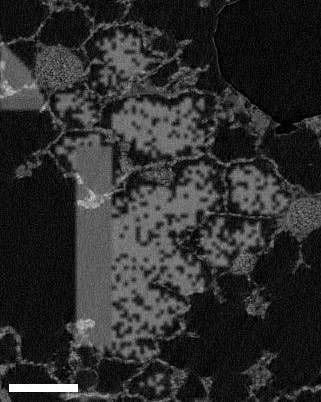
\includegraphics[height=\imsize]{img/Acini/2009f/mrg/R108C60Dt-mrg/acinus32/voxelsize1.48-every6slice/R108C60Dt-mrg-acinus32_45.png}% jpg is unedited!
		\label{subfig:60d_acinus32}%
	}%
	\hfill%
	\subfloat[60E, Acinus 38, Slice 29, Vol.\ \SI{188}{\percent}]{%
		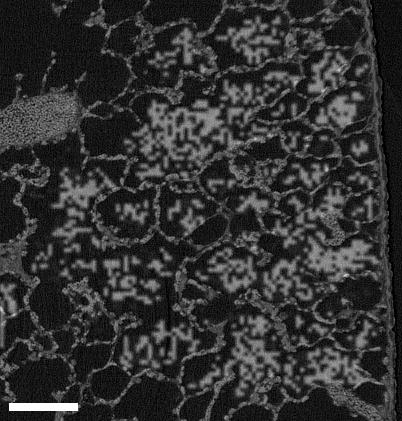
\includegraphics[height=\imsize]{img/Acini/2009f/mrg/R108C60Et-mrg/acinus38/voxelsize1.48-every6slice/R108C60Et-mrg-acinus38_29.png}% jpg is unedited!
		\label{subfig:60e_acinus38}%		
	}%
	\hfill%
	\caption{Illustrative slices of two acini that show large differences in volume between MeVisLab and STEPanizer. The inaccurate segmentation is the reason we obtained larger volumes with the STEPanizer than with MeVisLab. The image in panel \subref{subfig:60d_acinus32} shows minor segmentation errors through noise in the paraffin (dark spots inside grey region). The image in panel \subref{subfig:60e_acinus38} shows large segmentation errors. Such large errors arise through brightness changes in the dataset which render the global threshold unusable for certain slices. Scalebar: \SI{100}{\micro\meter}.}
	\label{fig:MeVisSegmentation}
\end{figure}

\subsection{Conclusions}
The hereby presented manhole cover method is well suited to semi-automatically isolate the functional lung units from three-dimensional datasets. The presented workflow permits a fully automated analysis of the volume of the functional lung units and enables the study of large amounts of acini in relatively short time.\todo{Shall we write something about the 1000 extracted acini for days \numrange{4}{60}?}

We validated our automatic method with a proven and accepted method, the so-called Stereology. We have shown that---even though there are slight differences between the two methods---the achieved results are comparable. Since our proposed method for assessing the volumes of isolated individual acini is by magnitudes faster than manual stereological counting, we believe the presented method is the easiest and fastest way to assess the volume of single functional units of mammalian lungs.

\clearpage
\section{Acknowledgments}
We thank Federica Marone, Beamline Scientist at TOMCAT for the long-standing great support at the Beamline and implementation of the reconstruction of the merged wide field scanning projections on the TOMCAT cluster. Christoph Hinterm\"{u}ller, former member of the TOMCAT group, and now at \href{http://gtec.at/}{g.tec medical engineering GmbH} also helped us during countless shifts at the beamline. He also helped with the first implementation of wide field scanning at TOMCAT. Bernd Pinzer, Post-Doc at TOMCAT adopted the support of our group from Chris and also does a fabulous job supporting us. Milo Hindennach, from Fraunhofer MEVIS provided the \href{http://www.mevis-research.de/cgi-bin/discus/board-auth.cgi?lm=1282233250&file=/839/11760.html}{Manhole cover module in MeVisLab}. We thank Mohammed Ouanella and Eveline Yao, our former and current lab technicians for expert technical assistance and embedding of the samples\todo{Oder ist Eveline Co-Autorin?}.

This work has been funded by the grants 3100A0-109874 and 310030-125397 of the Swiss National Science Foundation.

\clearpage
\singlespacing
\bibliographystyle{plainnat}
\bibliography{../references}

\end{document}